\section{Data generation pipeline}
\label{sec:data-generation}

\subsection{Benchmark design}
\label{subsec:benchmark-design}

The dataset is built around shared synthetic scenarios rather than solver-specific samples. Each scenario contains a procedurally generated bathymetry field, a synthetic initial-displacement source field, and metadata recording the sampled bathymetry family, source family, random strength factor, and file locations. Numerical reference trajectories are then produced by advancing the same scenario with one or more forward solvers. This separation between scenario generation and reference generation is important for multi-fidelity evaluation: when two solver labels differ, the difference is attributable to the numerical reference and not to a different random seabed or initial disturbance. Figure~\ref{fig:scenario-gallery} shows representative accepted scenario pairs spanning the morphology and source families described below.

The default forward benchmark uses a uniform $64 \times 64$ Cartesian grid on normalized coordinates, with matched bathymetry, source, and solver resolution. The training, validation, and test data come from three independently generated pools of $10{,}000$, $1{,}000$, and $2{,}500$ scenarios ($13{,}500$ in total), each produced by a separate generation run with its own fixed per-pool seed rather than by partitioning a single pool, so no scenario is shared between pools by construction; the processed splits are described in Section~\ref{subsec:preprocessing-targets}. Each trajectory is advanced for $250$ solver steps, every fifth state is saved, and the initial state is included, giving $51$ stored frames per rollout. Automatic time stepping is enabled with a target CFL value of $0.45$ for the shallow-water references. The default solver set now contains three references on the same scenario IDs: a hydrostatic-reconstruction shallow-water solver, a second-order MUSCL-HR shallow-water solver, and an elevation-only Boussinesq solver. Hydrostatic reconstruction remains the primary reference, while MUSCL-HR and Boussinesq provide two different comparison baselines for solver-fidelity analysis.

\begin{figure}[H]
\centering
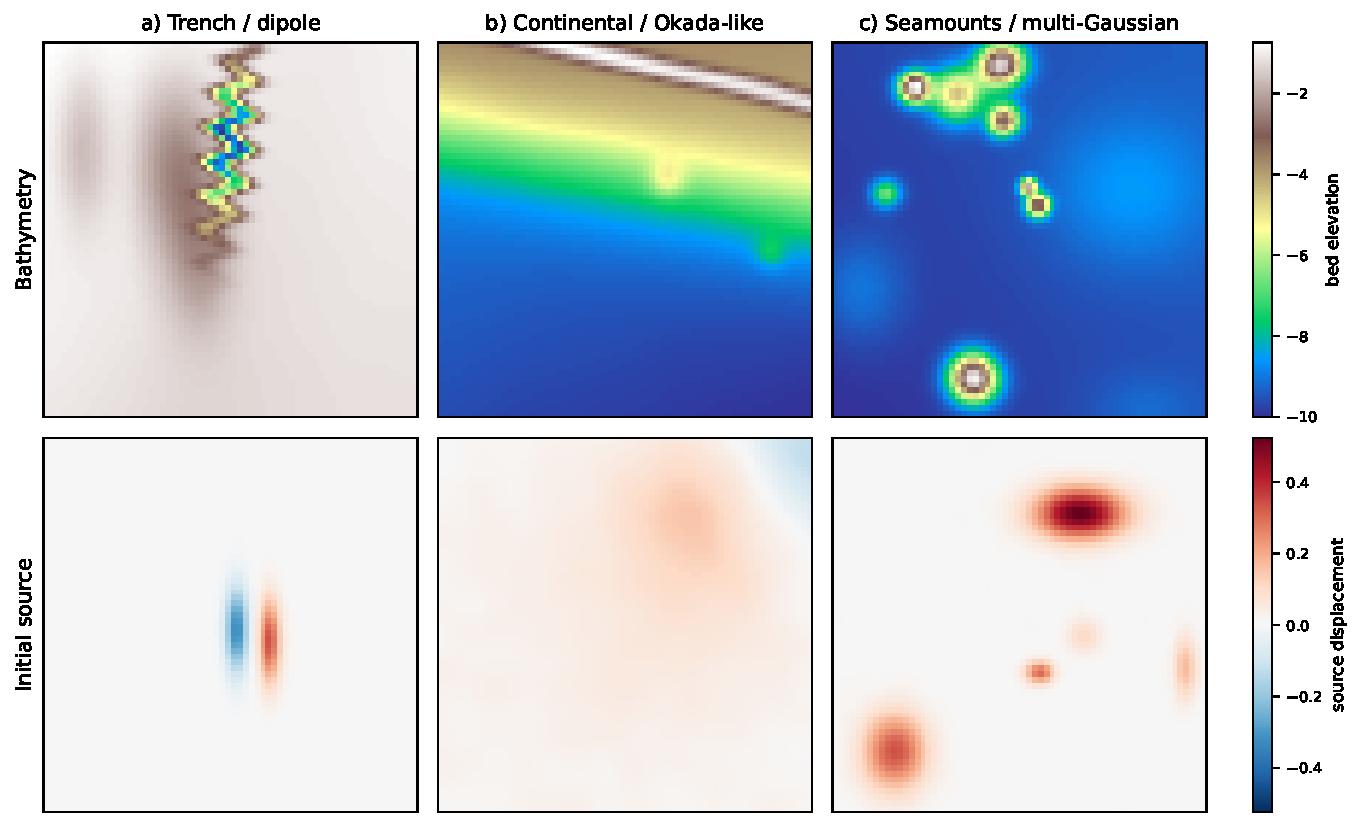
\includegraphics[width=0.6\linewidth]{figures/scenario_gallery.pdf}
\caption{Representative accepted synthetic scenarios from the benchmark generator. Each column shows one paired bathymetry/source scenario before rollout: trench/dipole, continental/Okada-like, and seamounts/multi-Gaussian. Bathymetry uses the shared fully wet range $[-10,-0.75]$; source fields retain family-dependent amplitudes and are shown on a shared symmetric uplift/subsidence scale.}
\label{fig:scenario-gallery}
\end{figure}

The benchmark is intentionally synthetic. Its purpose is to create a controlled supervised-learning problem for testing fast forward emulation of solver-generated tsunami-like wavefields, not to reproduce a specific coastline or to provide operational hazard assessment. This design makes it possible to evaluate solver fidelity, inference speed, distribution-shift behavior, cross-resolution transfer, and uncertainty quality under repeatable conditions.

\subsection{Procedural bathymetry}
\label{subsec:procedural-bathymetry}

Bathymetry is represented by a signed bed-elevation field $b(x,y)$, where $b(x,y)\leq 0$ denotes submerged cells below mean sea level. In the default configuration, every generated field is mapped into the range
\[
[d_{\min}, d_{\max}] = [-10, -0.75].
\]
This keeps the whole computational domain wet. The corresponding still-water depth is computed as
\[
h_{\mathrm{rest}}(x,y)=\max\{-b(x,y)+\eta_{\mathrm{sea}},0\},
\]
where $\eta_{\mathrm{sea}}$ is a configurable sea-level offset, set to zero in the default experiments.

For each scenario, the bathymetry generator samples one of five terrain families:
\[
\{\texttt{trench},\ \texttt{continental},\ \texttt{seamounts},\ \texttt{canyon},\ \texttt{island}\}.
\]
The generator first creates a low-frequency base field. In the current default configuration, this base is a weak rotated slope with slope components sampled from $[0.02,0.12]$, although flat and basin-like base modes are also supported. To reduce grid-aligned artifacts, the normalized coordinates are smoothly warped before the terrain-family morphology is evaluated:
\[
x_w=\operatorname{clip}(x+\alpha g_x(x,y),0,1),\qquad
y_w=\operatorname{clip}(y+\alpha g_y(x,y),0,1),
\]
where $g_x$ and $g_y$ are Gaussian-filtered random displacement fields and $\alpha$ is the configured warp scale.

The final unnormalized bathymetry is assembled as
\[
\tilde{b}(x,y)=b_{\mathrm{base}}(x,y)
+b_{\mathrm{family}}(x_w,y_w)
+\sum_i G_i(x,y)
+\sum_j R_j(x,y)
+N(x,y),
\]
where $b_{\mathrm{family}}$ is the dominant terrain-family term, $G_i$ are random Gaussian perturbations, $R_j$ are elongated ridge-like structures, and $N$ is multi-scale smoothed roughness. Trench and canyon samples emphasize elongated negative channels, seamount and island samples emphasize localized positive relief, and continental samples combine broad slopes with shelf-break-like structure. The stochastic Gaussian and ridge terms are sign-biased by family so that small-scale structure reinforces the selected morphology rather than erasing it.

After all components are combined, the field is min--max normalized and clipped:
\[
b(x,y)=d_{\min}
+\frac{\tilde{b}(x,y)-\min_{x,y}\tilde{b}}{\max_{x,y}\tilde{b}-\min_{x,y}\tilde{b}}
(d_{\max}-d_{\min}).
\]
This normalization deliberately prioritizes morphological diversity over site-specific amplitude realism. It also keeps the numerical problem bounded, which is useful when generating thousands of trajectories for model training. The procedural terrain construction follows the broader idea of synthetic terrain generation for controlled experiments, but the resulting fields should be interpreted as benchmark bathymetries rather than surveyed seafloor products \citep{musgrave1989terrain,sandwell2014gravity}.

\subsection{Initial-displacement sources}
\label{subsec:initial-displacement-sources}

The source generator produces an initial free-surface displacement template $\eta_{\mathrm{src}}(x,y)$ on the same grid as the bathymetry. The default source family set is
\[
\{\texttt{gaussian},\ \texttt{multi-gauss},\ \texttt{dipole},\ \texttt{fault},\ \texttt{rough},\ \texttt{okada-like}\}.
\]
Gaussian and multi-Gaussian sources provide localized smooth uplift patterns. Dipole sources create paired uplift and subsidence lobes. Fault sources create elongated rotated uplift structures. Rough sources are generated from smoothed random fields and broaden the distribution of source geometries. The \texttt{okada-like} family samples simplified fault parameters such as length, width, slip, angle, dip, and source depth, and constructs an anisotropic deformation pattern inspired by elastic half-space source models \citep{okada1985surface}. It is used only as a synthetic source family, not as a full geophysical rupture model.

In the default forward benchmark, per-sample source normalization is disabled. Thus each family preserves its sampled amplitude semantics instead of being forced into a common height interval. A separate independent strength factor
\[
s\sim\mathcal{U}(0.45, 0.85) % we lowered this so boussinesq can run on the same scenario ig
\]
is then applied during scenario construction to form the initial perturbation
\[
\eta_0(x,y)=s\,\eta_{\mathrm{src}}(x,y).
\]
The initial water depth passed to the shallow-water solvers is
\[
h_0(x,y)=\max\{h_{\mathrm{rest}}(x,y)+\eta_0(x,y),0\},
\]
and the horizontal momenta are initialized to zero. Therefore, each rollout starts from a displaced but initially motionless free surface over a synthetic seabed.

There is also a separate Boussinesq debugging configuration with smoother bathymetries, lower source amplitudes, and a smaller source-strength range. That file is useful for checking propagation plots, but it is not the main paper from the same bathymetry and source caches as the shallow-water solvers, so sample IDs stay aligned across targets.

\subsection{Reference rollouts and solver organization}
\label{subsec:reference-rollouts}

The primary reference labels are generated with finite-volume shallow-water solvers. The hydrostatic-reconstruction solver is used as the main reference because it enforces nonnegative depth and is designed to preserve lake-at-rest balance over non-flat bathymetry \citep{audusse2004hydrostatic}. The MUSCL-HR solver adds second-order reconstruction with hydrostatic reconstruction, giving a sharper comparison reference on the same scenarios. Both shallow-water references use Rusanov-type numerical fluxes, open boundary conditions, and a sponge layer near the boundary in the default configuration \citep{leveque2002finite,toro2009riemann,clain2016secondorder}.

For each shared scenario, enabled solvers write outputs into solver-specific sample folders, for example \path{data/raw/hydrostatic/samples} and \path{data/raw/muscl_hr/samples}. Each folder stores the full solver state trajectory, the reconstructed free-surface trajectory, timestamps, time-step history, and metadata. For the shallow-water solvers, the stored state contains depth and horizontal momentum components, while the free surface is reconstructed as
\[
\eta(x,y,t)=h(x,y,t)+b(x,y).
\]
For the Boussinesq solver, the first state channel is treated directly as the free-surface field. Scenario-level manifests record the shared scenario definition, while per-solver manifests record the corresponding numerical labels. This layout allows single-solver training, per-solver comparisons, and multi-fidelity preprocessing without resampling the underlying bathymetry-source pairs.

Quality checks are applied during generation before a sample is accepted. The default policy rejects non-finite states, depth violations below the configured tolerance, excessive free-surface amplitude, and excessive velocity. These checks are intended to prevent unstable or physically unusable rollouts from silently entering the supervised-learning labels.

\subsection{Preprocessing and learning targets}
\label{subsec:preprocessing-targets}

Preprocessing converts the raw rollout archives into model-ready arrays. The preprocessing code supports a default fixed-seed $70\%/15\%/15\%$ scenario split of a single pool, but for the experiments in this paper we deliberately choose a stronger design and generate the training, validation, and test pools as independent runs. The training pool uses $10{,}000$ scenarios, the validation pool $1{,}000$, and the test pool $2{,}500$. The validation and test pools are generated with separate fixed dataset seeds, so their per-sample random seeds differ even when the sample indices start again from one. This guarantees that no scenario is shared between the pools by construction, rather than relying on a random partition. The same scenario design is reused across solver targets, so the hydrostatic, MUSCL-HR and Boussinesq datasets can be compared without changing the underlying bathymetry-source pairs.

The default input channels are bathymetry, source field, and initial water depth. The initial free surface can also be exported as an ablation channel, and a scalar solver-identity channel is available for explicit multi-fidelity experiments. The default target variable is the free-surface elevation $\eta$. With the default rollout settings, preprocessing discards the stored initial frame from the prediction target and keeps the next $50$ saved frames as a multi-step forecast target.

Normalization statistics are computed from the training split only and then reused unchanged for validation and test samples. The default method is standardization for the active input channels and trajectory targets. Processed evaluation archives additionally retain sample identifiers, bathymetry type, source type, solver name, source strength, and normalization information. These metadata are used by the evaluation scripts to report aggregate accuracy as well as grouped metrics under distribution-shift suites.

\subsection{Distribution-shift and resolution-transfer datasets}
\label{subsec:shift-resolution-data}

The same metadata-first design supports controlled generalization tests. For source-family shift, bathymetry-family shift, and source-strength shift, the evaluation pipeline builds filtered suites from the processed test archives using metadata such as \texttt{source\_type}, \texttt{bathymetry\_type}, and \texttt{source\_strength}. In the current configuration, these suites include a multi-Gaussian source subset, a trench bathymetry subset, and a high-source-strength subset. When reporting a strict held-out-family experiment, the corresponding family should be excluded from the training split before preprocessing and then evaluated through the same metadata-filtered suite. This distinction avoids confusing a difficult subgroup evaluation with a truly unseen-family generalization test.

For cross-resolution transfer, we additionally generate native $32\times32$ and $128\times128$ test pools of $1{,}000$ scenarios each, alongside the main $64\times64$ data. These pools keep the same procedural generation logic while changing the grid spacing, the sponge width, and, for the finest grid, the target CFL value. The shared-from-$64$ preprocessing mode can force the lower- and higher-resolution datasets to use normalization statistics from the $64\times64$ training distribution. This gives a stricter transfer setting: the model is evaluated on a changed grid resolution without recomputing the feature scaling from the target resolution.
